\chapter{Introduction}

\section{Introducing \packageName}

{\packageName} is a multi-scale model of \textit{in silico} experimental evolution, the virtual pendant of experimental evolution in wet laboratory (see Fig~\ref{general_algorithm}).
The software is equiped with the whole tool case of experimental setups, competition assays, phylogenetic analysis, and, most importantly, allowing for evolvable ecological interactions. Digital organisms with an evolvable genome structure, encoding evolvable genetic regulation and metabolic networks are evolved for tens of thousands of generations in environments mimicking the dynamics of real controlled environments, including chemostat or batch culture.

{\packageName} was developed under \textsc{EvoEvo} (\href{http://www.evoevo.eu/}{http://www.evoevo.eu/}), a FP7-ICT project funded by the European Commission (FP7-ICT-610427). The source code is written in C++.

You can find more details on software description and development on Github page charlesrocabert/Evo2Sim. A website fully dedicated to {\packageName} is coming soon.

\section{License}

This program is free software: you can redistribute it and/or modify it under the terms of the GNU General Public License as published by the Free Software Foundation, either version 3 of the License, or (at your option) any later version.

This program is distributed in the hope that it will be useful, but WITHOUT ANY WARRANTY; without even the implied warranty of MERCHANTABILITY or FITNESS FOR A PARTICULAR PURPOSE. See the GNU General Public License for more details.

You should have received a copy of the GNU General Public License along with this program. If not, see \href{http://www.gnu.org/licenses/}{http://www.gnu.org/licenses/}.

\section{Community}
{\packageName} was developed by Charles Rocabert, Carole Knibbe and Guillaume Beslon, under the \textsc{EvoEvo} project. The list of contributors is displayed in text-file \texttt{AUTHORS} of {\packageName}  package.
You shall find more details on \href{http://www.evoevo.eu/community/}{http://www.evoevo.eu/community/}.

\section{Download}
{\packageName} last releases are available on Github page charlesrocabert/Evo2Sim.

\section{Contact}
For any question about the software, do not hesitate to contact us at\\ \href{http://www.evoevo.eu/contact-us/}{http://www.evoevo.eu/contact-us/}.

\newpage
\thispagestyle{empty}

\begin{figurehere}
\centering 
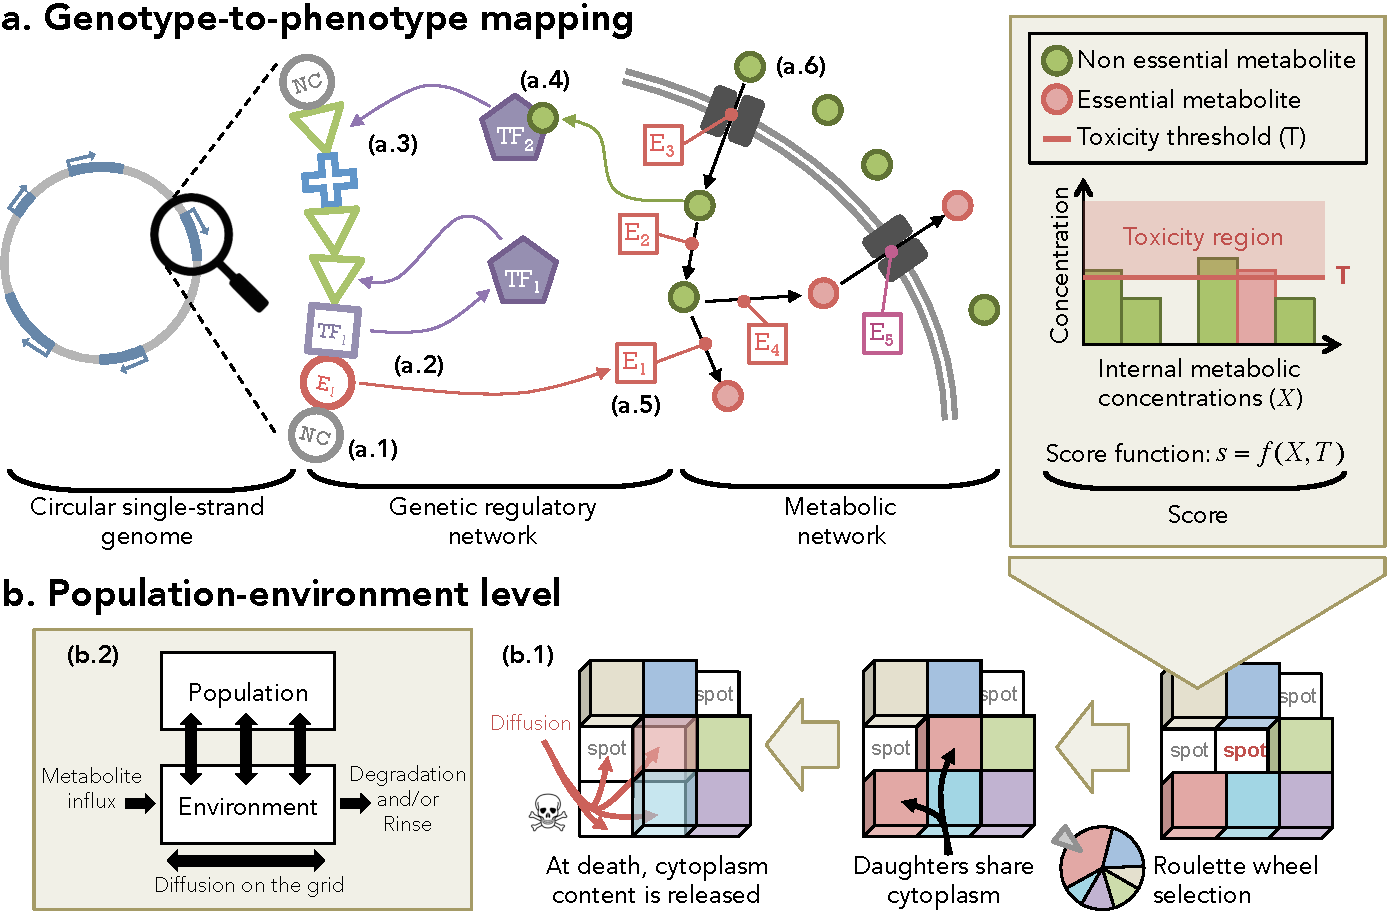
\includegraphics[width=0.95\textwidth]{figures/general_algorithm.pdf}
\caption[Global picture of {\packageName}.]{\small{\textbf{Global picture of {\packageName}.} \textbf{a. Description of the genotype-to-phenotype mapping.} Organisms own a coarse-grained genome made of units. This genome is a circular single-strand sequence, with a unique reading frame. Non coding \textbf{(NC)} units are not functional \textbf{(a.1)}. The arrangement of the units on the sequence defines functional regions, where a promoter (\textbf{P}, blue cross) controls the expression of enzyme coding units (\textbf{E}, red circles) or transcription factor coding units (\textbf{TF}, purple squares), thereby allowing for operons (here, one E and one TF). When coding units are expressed \textbf{(a.2)}, they contribute to the genetic regulatory network (for TFs) and the metabolic network (for Es).
Depending on their attributes, transcription factors bind on binding sites. \textbf{(a.3)} If they bind on the enhancer sequence (binding sites flanking the promoter upstream), the promoter activity is up-regulated. If they bind on the operator sequence (binding sites flanking the promoter downstream), the promoter activity is down-regulated. \textbf{(a.4)} Metabolites can bind on a transcription factor as co-enzymes, and activate or inhibit it, depending on transcription factor attributes.
Enzymes perform metabolic reactions in the cytoplasm \textbf{(a.5)}, or pump metabolites in or out \textbf{(a.6)}. The score of an organism is computed from its ``essential metabolites''
(usually the score is the sum of essential metabolite concentrations). Lethal toxicity thresholds are applied to each metabolic concentration and forbid organisms to accumulate resources. \textbf{b. Description of the population and environment levels.} Organisms are placed on a 2D toroidal grid, and compete for resources and space. When an organism dies, it leaves its grid cell empty and organisms in the Moore neighborhood (if any) compete to divide in available space. The competition is based on scores, a minimal threshold being applied on scores to forbid worst organisms to divide. At division, daughters share cytoplasm content (enzymes and metabolites). At death, metabolites from the cytoplasm are released in the local environment, and diffuse on the grid \textbf{(b.1)}. On the largest scale, the population evolves on the environment by up-taking, transforming and releasing metabolites. Metabolites then diffuse and are degraded. This strong interaction between the population and the environment allows for the evolution of complex ecological situations, depending on environmental properties \textbf{(b.2)}.}}
\label{general_algorithm}
\end{figurehere}


